\documentclass{beamer}

\usepackage[utf8]{inputenc}
\usepackage[english]{babel}

\usepackage{amsmath}
\usepackage{nicefrac}

\usepackage{minted}
\usepackage{fontspec}

\usepackage{xcolor}
\usepackage{graphicx}

\usemintedstyle{friendly}
\setmonofont{Source Code Pro}
\usetheme{metropolis}

\newminted{rust}{escapeinside=||, fontsize=\footnotesize, bgcolor=bg, autogobble, rust}
\newminted{java}{escapeinside=||, fontsize=\footnotesize, bgcolor=bg, autogobble, java}

\newcommand{\then}{\Rightarrow}

\title{Bounded generics over constants in Rust}
\author{Author: Christian Poveda \\ Advisor: Nicolás Cardozo}
\institute{Systems and Computing Engineering Department \\ Universidad de los Andes}
\date{2018-09-18}

\begin{document}

\frame{\titlepage}

\begin{frame}[fragile]
    \frametitle{Context: What is a type?}
    On this snippet
    \begin{javacode}
        String myString = "Hello, World!";
    \end{javacode}
    we would say \texttt{\footnotesize String} is the type of \texttt{\footnotesize myString} and as such, it determines:
    \begin{itemize}
        \item The operations on which \texttt{\footnotesize myString} could be used.
        \item The values \texttt{\footnotesize myString} could take.
        \item The type of \texttt{\footnotesize "Hello, World!"} (it should be \texttt{\footnotesize String}).
    \end{itemize}
\end{frame}

\begin{frame}[fragile]
    \frametitle{Context: What is a type?}
    To be more specific: 
    \begin{center}
        \textit{A type system is a syntatic method for proving the absence of certain program behaviors by classifying phrases according to the kinds of values they compute}
    \end{center}
    Usually type systems are described using \textit{typing rules}:
    $$true &: \texttt{\footnotesize Bool}$$ 
    $$false &: \texttt{\footnotesize Bool}$$ 

    $$\frac{t_1 : \texttt{\footnotesize Bool}\ t_2 : T\ t_3 : T}{\texttt{\footnotesize if}\ t_1\ \texttt{\footnotesize then}\ t_2\ \texttt{\footnotesize else}\ t_3\ : T}$$
\end{frame}

\begin{frame}[fragile]
    \frametitle{Context: The Rust programming language}
    Rust is a systems programming language focused on safety, speed and concurrency. However, Rust is not your typical language:
    \begin{itemize}
        \item It is blazingly fast (almost as fast as C++).
        \item It has high-level features:
            \begin{itemize}
                \item Pattern matching
                \item Traits
                \item Higher order functions
            \end{itemize}
        \item It does not have garbage collection nor pointer arithmetic, but it is memory safe.
        \item It features concurrency without data races.
    \end{itemize}
\end{frame}

\begin{frame}[fragile]
    \frametitle{Context: Rust's type system}
    Rust's type system is based on the ML type system and it has
    \begin{itemize}
        \item \textbf{Static type checking:} Programs are checked for safety during compilation.
        \item \textbf{Type inference:} Type annotations are not always needed.
        \item \textbf{Polymorphism}  via traits and generics.
        \item \textbf{Algebraic data types:} It has enums and structs.
    \end{itemize}
    It also takes care of memory safety
    \begin{itemize}
        \item Rust encodes the lifetime of each variable in its type.
        \item For each variable, Rust only allows one of the following:
            \begin{itemize}
                \item One mutable reference.
                \item Several inmutable references.
            \end{itemize}
    \end{itemize}
\end{frame}

\begin{frame}[fragile]
    \frametitle{The problem: Functions over arrays}
    In Rust:
    \begin{itemize}
        \item Arrays (being stack allocated) must be statically sized.
        \item Writing functions or traits for arrays is cumbersome.
    \end{itemize}
    As a consequence, this code compiles
    \begin{rustcode}
    fn add_arr(a: &[f64; 3], b: &[f64; 3]) -> [f64; 3] {
        let mut result = [0.0; 3];
        for i in 0..3 {
            result[i] = a[i] + b[i];
        }
        result
    }
    \end{rustcode}
\end{frame}

\begin{frame}[fragile]
    \frametitle{The problem: Functions over arrays}
    In Rust:
    \begin{itemize}
        \item Arrays (being stack allocated) must be statically sized.
        \item Writing functions or traits for arrays is cumbersome.
    \end{itemize}
    But this code does not
    \begin{rustcode}
    fn add_arr(a: &[f64; N], b: &[f64; N]) -> [f64; N] {
        let mut result = [0.0; N];
        for i in 0..N {
            result[i] = a[i] + b[i];
        }
        result
    }
    \end{rustcode}
\end{frame}

\begin{frame}[fragile]
    \frametitle{The solution: Constant values as type parameters}
\end{frame}

\begin{frame}[fragile]
    \frametitle{The result: Arrays as const-generic types}
    With generics over constant values, we can write traits and functions for any array size
    \begin{rustcode}
    fn add_arr <const N: usize> (
        a: &[f64; N],
        b: &[f64; N]
    ) -> [f64; N] {
            let mut result = [0.0; N];
        for i in 0..N {
            result[i] = a[i] + b[i];
        }
        result
    }
    \end{rustcode}
    However, this adds a new problem about constant values as parameters
\end{frame}

\begin{frame}[fragile]
    \frametitle{The problem: Checking bounds}
    Even if we had generics over constant values, we still have to do dynamical checks for constant values 
    \begin{rustcode}
        fn <const N: usize> head(a: [f64; N]) -> Option<f64> {
            if N > 0 {
                Some(a[0])
            } else {
                None
            }
        }
    \end{rustcode}
    Even though the compiler has the value for  \texttt{N} (it is a constant), we are doing checks over \texttt{N} at run-time.
\end{frame}

\begin{frame}[fragile]
    \frametitle{The solution: Bounds over value parameters}

\end{frame}

\begin{frame}[fragile]
    \frametitle{The result: Checking bounds}
    Now, we can write static bounds over constant parameters.
    \begin{rustcode}
        fn <const N: usize> head(a: [f64; N]) with {N > 0} -> f64 {
            a[0]
        }
    \end{rustcode}
    Given that the bound \texttt{\footnotesize N > 0} is checked during compilation and not in run-time. This code is not just shorter, is faster.
\end{frame}

\begin{frame}[fragile]
    \frametitle{Context: Generics over values in theory}
    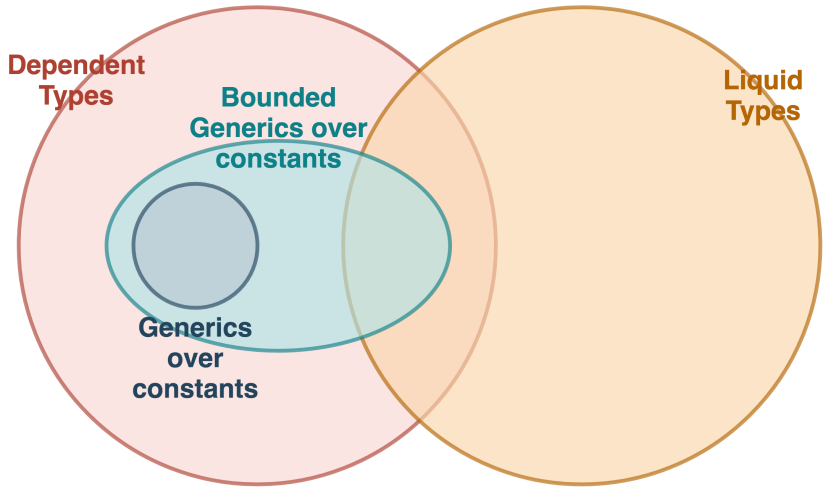
\includegraphics[width=\textwidth]{./theory.png}
\end{frame}

\begin{frame}[fragile]
    \frametitle{Context: Languages with dependent/liquid types}
    Haskell, Idris, Agda, Coq, Otros. Mostrar número de papers en el último año para cada uno
\end{frame}

\begin{frame}[fragile]
    \frametitle{Context: Idris, a dependently typed language}
    Como se ve Idris y que deja hacer
\end{frame}

\begin{frame}[fragile]
    \frametitle{Context: Rust Status Quo}
    RFC-2000, que hay, que habrá y que quedará faltando
\end{frame}

\begin{frame}[fragile]
    \frametitle{Road Ahead: What needs to be done}
    Desbaratar los ejemplos para mostrar que pasos hay que seguir, entre ellos unificación
\end{frame}

\begin{frame}[fragile]
    \frametitle{Road Ahead: Unification}
    Mostrar que alternativas hay para implementarla
\end{frame}

\begin{frame}[fragile]
    \frametitle{Validation: Formal verification}
    Proveer una prueba formal de que unificación y bounds son bien comportados 
\end{frame}

\begin{frame}[fragile]
    \frametitle{Validation: Comparison against other languages}
    Con estas nuevas features hasta donde puede dar Rust al compararlo con lenguajes como Idris
\end{frame}

\begin{frame}[fragile]
    \frametitle{Validation: Integration with Rust}
    Integrar este trabajo dentro de Rust como tal, RFCs y PRs al respecto
\end{frame}

\begin{frame}[fragile]
    \frametitle{Schedule}
    El cronograma... para (no) cumplirlo
\end{frame}
